\documentclass[12pt]{article}
\usepackage[margin=1in]{geometry}
\usepackage[spanish,es-lcroman]{babel}
\usepackage{amsmath,amsthm,amssymb,amsfonts}
\usepackage{graphicx}

\newcommand{\Cp}{\texttt{C+-}}
\newcommand{\C}{\texttt{C}}
\newcommand{\Cpp}{\texttt{C++}}

\newenvironment{problem}[2][Problem]{\begin{trivlist}
\item[\hskip \labelsep {\bfseries #1}\hskip \labelsep {\bfseries #2.}]}{\end{trivlist}}
%If you want to title your bold things something different just make another thing exactly like this but replace "problem" with the name of the thing you want, like theorem or lemma or whatever


\begin{document}

%\renewcommand{\qedsymbol}{\filledbox}
%Good resources for looking up how to do stuff:
%Binary operators: http://www.access2science.com/latex/Binary.html
%General help: http://en.wikibooks.org/wiki/LaTeX/Mathematics
%Or just google stuff

\title{Reporte 1. Lenguaje C+-}
\author{Mat\'ias Greco, Javier Reyes}
\date{2 de Octubre, 2018}
\maketitle

\section*{Introducci\'on}
El presente reporte explica el trabajo realizado para el desarrollo de un anailzador l\'exico y sint\'actico para el lenguaje de programaci\'on \Cp.

El lenguaje \texttt{C+-} corresponde a un subconjunto del lenguaje \C, con la adici\'on de algunas caracter\'isticas de \Cpp, como la posibilidad de definir una funci\'on con paso por valor o paso por referencia.

El analizador l\'exico y sint\'actico fue desarrollado en la herramienta ANTLR4 (ANother Tool for Language Recognition) con lenguaje de salida \Cpp.

El repositorio del proyecto está disponible en github\footnote{https://github.com/matgreco/Cmm-Compiler}.


\section*{Caracter\'isticas del lenguaje}

El lenguaje \texttt{C+-} incluye las siguientes caracter\'isticas, propias del standard \texttt{C89}
\begin{itemize}
    \item Funciones.
    \item Declaraciones.
    \item Asignaciones.
    \item Expresiones l\'ogicas y de operaciones.
    \item If.
    \item Switch (case y default).
    \item While.
    \item For.
    \item Do While.
    \item Struct.
\end{itemize}

Algunas caracter\'isticas interesantes incluidas:
\begin{itemize}
    \item Comma expression
\end{itemize}

\subsection*{Caracter\'iticas no incluidas}
\begin{itemize}
    \item Macros:

    No se incluy\'o debido a que complica todo el proceso. Requerir\'ia una precompilaci\'on y la capacidad de incluir otros archivos mediante enlazado.
    \item Punteros:

    No se incluy\'o debido a que complica la gram\'atica, por la aparici\'on de una infinidad de tipos distintos (del estilo \texttt{int***}). Tambi\'en requiere una administraci\'on de memoria que se escapa un poco de nuestro objetivo.

    \item Typedef:

    No se incluy\'o debido a que complica la gram\'atica. Eso permitir\'ia utilizar una expresi\'on de tipo \texttt{VAR} como una definici\'on de tipo. Al no incluirlo, el lenguaje no pierde capacidades, ya que una estructura personalizada \texttt{S} tiene tipo \texttt{struct S}.
\end{itemize}

\subsection*{Definiciones l\'exicas}

La definici\'on de los componentes l\'exicos del lenguaje \texttt{C+-} es similar al lenguaje \C, y se define de la siguiente forma:
\begin{itemize}
    \item \textbf{Keywords:} \texttt{int}, \texttt{char}, \texttt{double}, \texttt{float}, \texttt{long}, \texttt{short}, \texttt{unsigned}, \texttt{sizeof}, \texttt{if}, \texttt{else}, \texttt{while}, \texttt{for}, \texttt{break}, \texttt{continue}, \texttt{true}, \texttt{false}, \texttt{struct}, \texttt{void}, \texttt{return}, \texttt{switch}, \texttt{case}, \texttt{default}, \texttt{do}. Tienen el mismo uso que en \C.
    \item \textbf{Identificadores:} Puede componerse de letras, n\'umeros y guiones bajos, pero no pueden empezar con un n\'umero.
    \item \textbf{Valores constantes:} Pueden ser n\'umeros enteros con o sin signo (expresables en base 8, 10 y 16), n\'umeros de punto flotante, caracteres y strings.
    \item \textbf{Operadores aritm\'eticos:} \texttt{+} para suma, \texttt{-} para resta, \texttt{*} para multiplicaci\'on \texttt{/} para divisi\'on y \texttt{\%} para el resto de la divisi\'on.
    \item \textbf{Operadores de comparaci\'on:} \texttt{==}, \texttt{!=}, \texttt{<=}, \texttt{>=}, \texttt{<}, \texttt{>}.
    \item \textbf{Operadores unarios:} \texttt{++}, \texttt{--}, \texttt{+}, \texttt{-}, \texttt{!}, $\mathtt\sim$.
    \item \textbf{Operadores de shift:} \texttt{<{}<}, \texttt{>{}>}.
    \item \textbf{Operadores bitwise:} \texttt{\&}, \texttt{\^}, \texttt{|}.
    \item \textbf{Operadores l\'ogicos:} \texttt{\&\&}, \texttt{||}.
    \item \textbf{Operador ternario:} \texttt{ ? : }
    \item \textbf{Operador coma:} \texttt{exp1,exp2} ejecuta \texttt{exp1}, luego \texttt{exp2} y retorna \texttt{exp2}.
    \item \textbf{Operadores varios:} \texttt{sizeof} retorna el tama\~no en bytes de una expresi\'on o tipo; llamadas a m\'etodos (\texttt{f(exp1,exp2)}); acceso a miembros (\texttt{estructura.miembro}); y acceso a elementos de un array (\texttt{arr[i]}).
\end{itemize}

\subsection*{Resoluci\'on de ambig\"uedades y precedencias}

Las ambig\"uedades presentes en el lenguaje son
\begin{itemize}
    \item Problema If/If/Else: En este caso, si se da
    \begin{verbatim}
    if(exp1) if(exp2) st1; else st2;
    \end{verbatim}
    el \texttt{else} corresponde siempre al \texttt{if} m\'as al interior, es decir, es equivalente a
    \begin{verbatim}
    if(exp1)
    {
        if(exp2)
        {
            st1;
        }
        else
        {
            st2;
        }
    }
    \end{verbatim}
    \item Problemas del estilo
    \begin{verbatim}
    a = b ? c : d = e;
    \end{verbatim}
    En este caso, el standard no determina si el orden debe ser
    \begin{verbatim}
    a = (b ? c : (d = e));
    \end{verbatim}
    o bien
    \begin{verbatim}
    a = ((b ? c : d) = e);
    \end{verbatim}
    Por lo tanto, dejamos este problema como \textit{undefined behavior}.
\end{itemize}

Las precedencias son las standard para \texttt{C} y para lenguajes de programaci\'on similares.

\section*{Pruebas}
En el repositorio se encuentras siete c\'odigos de prueba, dos de los cuales arrojan errores con la intenci\'on de probar el funcionamiento del analizador l\'exico.
Una de las pruebas mas sencillas que se realiz\'o fue utilizando el c\'odigo siguiente, donde se muestran una llamada a una funci\'on (la funci\'on principal), declaraciones, asignaciones y la utilizaci\'on del operador coma. 
\begin{verbatim}
int main()
{
    int a = 10;
    int b = 30;
    int c;
    
    c = a,b,a;
    
    printf("%d",c);

    return 0;
}
\end{verbatim}
Este c\'odigo, al pasar por el analizador l\'exico y sint\'actico, arroja el AST dispuesto en la figura 1.


\centerline{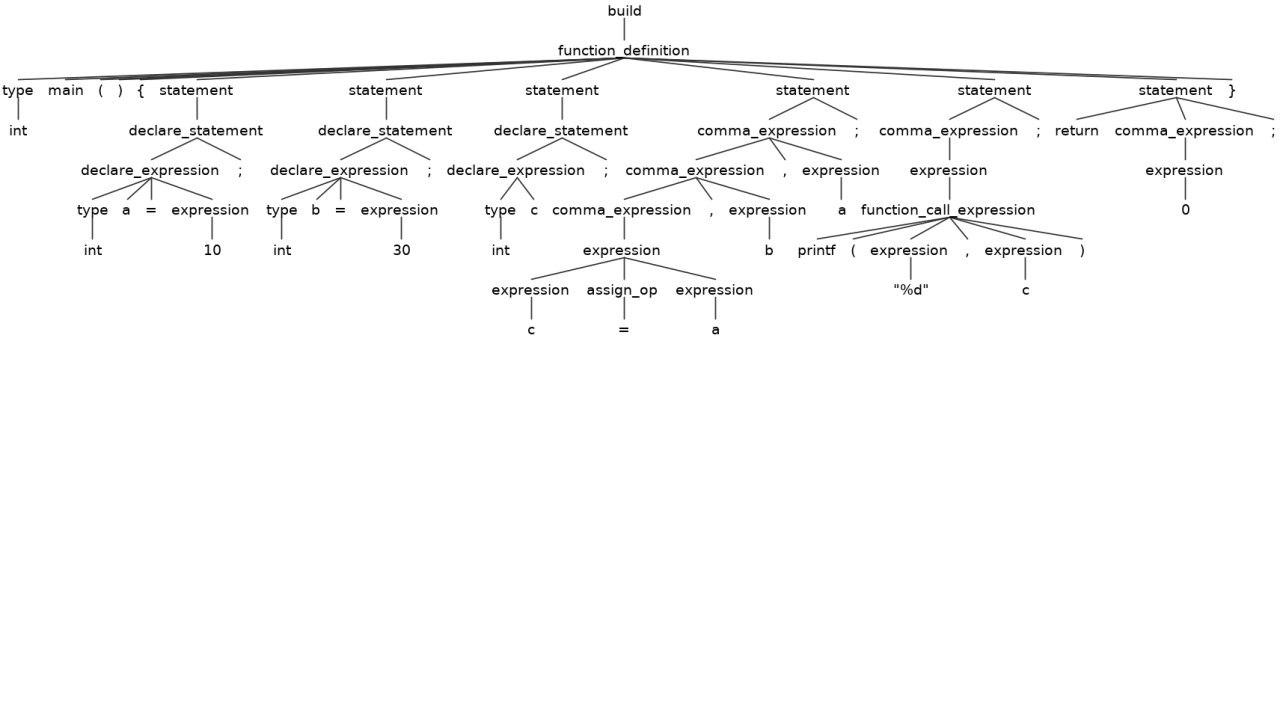
\includegraphics[trim={0 9cm 0 0},scale=0.45]{arbol1.jpg}}
\centerline{Figura 1: AST obtenido.}
\clearpage

\section*{Conclusiones}
En este reporte se presentó la definición de la gramática para el subconjunto del lenguaje C llamado C+-. Este trabajo fue realizado utilizando ANTLR4, el cual permitió facilmente diferenciar entre reglas sint\'a cticas y tokens a trav\'es de la utilizaci\'on de may\'usculas.

\section*{Ap\'endice 1: Toda la gram\'atica}
Antes que todo, cabe resaltar que si bien esta gram\'atica no es LL(*) dado que tiene recursiones por la izquierda, ANTLR4 es capaz de reconocer algunas de estas recursiones y por detras las modifica para que la gram\'atica resultante sea efectivamente LL(*). Por ejemplo, para la variable \texttt{expression}, la modificaci\'on es escencialmente la misma que agregar tantos niveles asociados a expresiones como prioridades para operaciones hay.
\begin{verbatim}
grammar Cmm2;

build:
    (
        declare_statement
        | forward_function_definition
        | function_definition
        | struct_definition
        | ';'
    )*
;

declare_statement:
    declare_expression ';'
;

declare_expression:
    type VAR ('=' expression)? (',' VAR ('=' expression)?)*
    | type VAR '[' comma_expression ']'
;

compare_op:
    '=='
    | '<='
    | '>='
    | '<'
    | '>'
;

assign_op:
    '='
    | '+='
    | '-='
    | '*='
    | '/='
    | '%='
    | '<<='
    | '>>='
    | '&='
    | '^='
    | '|='
;

unary_left_op:
    '++'
    | '--'
    | '+'
    | '-'
    | '!'
    | '~'
;

statement:
    comma_expression?';'
    | declare_statement
    | Break ';'
    | Continue ';'
    | Return comma_expression? ';'
    | Case INT_NUMBER ':'
    | Default ':'
    | if_statement
    | while_statement
    | for_statement
    | switch_statement
    | do_statement
    | '{' statement* '}' 
;

if_statement:
    If '(' comma_expression ')' statement (Else statement)?
;

switch_statement:
    Switch '(' comma_expression ')' '{' statement* '}'
;

while_statement:
    While'(' comma_expression ')' statement
;

for_statement:
    For '('
    (comma_expression | declare_expression)? ';'
    comma_expression? ';'
    comma_expression?
    ')' statement
;

do_statement:
    Do statement While '(' comma_expression ')' ';'
;


function_call_expression : 
    VAR '(' (expression (',' expression)*)? ')'  
;

function_definition : 
    (type | 'void') VAR '('
    ((type '&'? VAR (',' type '&'? VAR)*)? | 'void')
    ')' '{' statement* '}'  
;

forward_function_definition:
    (type | 'void') VAR '('
    ((type '&'? VAR? (',' type '&'? VAR?)*)? | 'void')
    ')' ';'
;

struct_definition:
    'struct' VAR '{'
        declare_statement*
    '}' ';'
;

FLOAT_NUMBER :
    [0-9]* '.' [0-9]+
    | [0-9]+ '.' [0-9]*
;

INT_NUMBER:
    DEC_NUMBER ('u' | 'U')? ('ll' | 'LL')?
    | OCT_NUMBER ('u' | 'U')? ('ll' | 'LL')?
    | HEX_NUMBER ('u' | 'U')? ('ll' | 'LL')?
    | CHAR_CONSTANT
;

STRING_CONSTANT :
    '"' ~('"')* '"'
;

CHAR_CONSTANT:
    '\'' ~('\'')* '\''
;


DEC_NUMBER:
    '0'
    | [1-9][0-9]*
;

OCT_NUMBER:
    '0'[0-7]+
;

HEX_NUMBER:
    ('0x' | '0X')[0-9a-fA-F]+
;

type:
    Unsigned? Int
    | Unsigned? Char
    | Double
    | Unsigned? Long
    | Unsigned? Short
    | Float
    | 'struct' VAR
;

//KEYWORDS
Int:'int';
Char:'char';
If:'if';
Else:'else';
While:'while';
For:'for';
Break:'break';
Continue:'continue';
True:'true';
False:'false';
Struct:'struct';
Void:'void';
Return:'return';

Switch:'switch';
Case:'case';
Default:'default';
Do:'do';

Double:'double';
Long:'long';
Short:'short';
Float:'float';
Unsigned:'unsigned';
Sizeof:'sizeof';

VAR:
    [a-zA-Z_][a-zA-Z0-9_]*
;


WS
    : [ \t\u000C\r\n]+ -> skip
;

COMMENT:
    '//' ~[\n]* -> skip
;

MULTILINE_COMMENT:
    '/*' .*? '*/' -> skip
;

comma_expression:
    expression
    | comma_expression ',' expression
;

expression:
    '(' comma_expression ')'
    | INT_NUMBER
    | STRING_CONSTANT
    | CHAR_CONSTANT
    | FLOAT_CONSTANT
    | VAR
    | expression '.' VAR
    | 'sizeof' '(' (expression | type) ')'
    | function_call_expression
    | expression '[' expression ']'
    | expression ('++' | '--')
    | unary_left_op expression
    | expression ('*' | '/' | '%') expression
    | expression ('+' | '-') expression
    | expression ('<<' | '>>') expression
    | expression ('<' | '<=' | '>' | '>=') expression
    | expression ('==' | '!=') expression
    | expression '&' expression
    | expression '^' expression
    | expression '|' expression
    | expression '&&' expression
    | expression '||' expression
    | <assoc=right> expression '?' comma_expression ':' expression
    | <assoc=right> expression assign_op expression
;
\end{verbatim}



\end{document}